\section{Evaluation Results}\label{result}

This section presents quantitative evaluation results of the proposed adaptive-precision ADC 
designs, including a column-parallel Single-Slope (SS) ADC and a column-parallel successive 
approximation register (SAR)/SS ADC. Both ADC designs are implemented using TSMC 65nm processing,
and simulated in Virtuoso’s AMS Environment. Circuit power consumption is collectively estimated
based on the average transient current of different ADC modules given one complete sampling and 
conversion period. Power savings are then estimated by comparing the power consumption of the
low-precision conversion mode against that of the high-precision conversion mode. 

\subsection{Evaluation of the SS ADC design}
Table~\ref{tab1} summarizes the key design characteristics of the SS ADC design. Considering a 
$512\times512$ pixel array, the frame rate is 162fps.  The SNDR of the SS ADC is 23.83/46.64 dB, 
which means the ENOB is 3.67/7.46 bits.  The power consumption of the SS ADC is measured and 
divided by column. It shows that the power consumption of the low-precision conversion mode is 
40.8uW/column, and the power consumption of the high-precision conversion mode is 76.2uW/column. 
Compared to the high-precision conversion mode, the low-precision conversion mode can reduce 
the power consumption approximately 50\%. Detailed power breakdown is shown in Fig.~\ref{SSresults1},
which demonstrates that the power consumption of the SS ADC design is mainly contributed by 
the  column-parallel comparators and the output buffer of the ramp generator, both of which 
can be effectively regulated via power gating for low-power conversion. The power consumption
results are also presented in Fig.~\ref{SSresults2}. The peripheral circuits include a bandgap 
and voltage divider, level-shift circuits and global buffers.

\begin{table}[htbp]
	\caption{Performance of the SS ADC design}
	\begin{center}
		\begin{tabular}{|c|c|}
			\hline
			\textbf{Prameter}& \textbf{Value} \\
			\hhline{|==|}
			\textbf{Process}& 65nm \\
			\hline 
			\textbf{Supply voltage}& 2.5/1.2 V \\
			\hline
			\textbf{Clock Frequency}&	25MHz \\
			\hline
			\textbf{Architecture}&	SS \\
			\hline
			\textbf{Quantization bits}&	4/8 bits\\
			\hline
			\textbf{Conversion time}&	12.04us \\
			\hline
			\textbf{Number of parallel columns}&	512 \\
			\hline
			\textbf{Throughput (samples per second)}&	42.5M \\ 
			\hline
			\textbf{Power (per column)}&	40.8/76.2 uW \\
			\hline
			\textbf{SNDR}& 23.83/46.64 dB@ 8.44 kHz\\
			\hline
			\textbf{ENOB}& 3.67/7.46 bits\\
			\hline
			\textbf{FOM$^{\mathrm{a}}$}& 38.59/5.21 pJ/step\\
			\hline
			\multicolumn{2}{l}{$^{\mathrm{a}}\textbf{FOM}=(\textbf{Power}\ast \textbf{Conversion}\ \textbf{time})/2^{\textbf{ENOB}}$ }	    
		\end{tabular}
		\label{tab1}
	\end{center}
\end{table}

\begin{figure}[htbp]
	\centerline{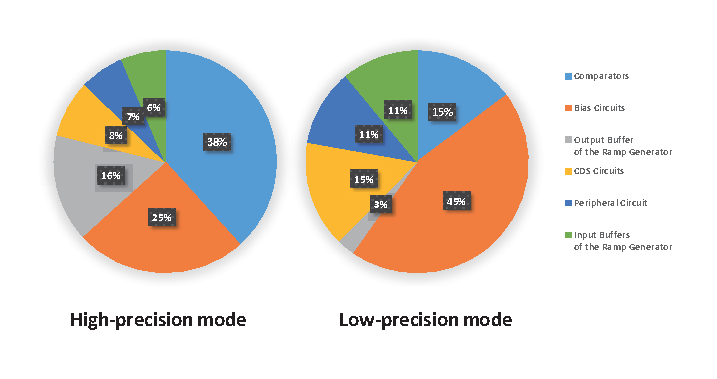
\includegraphics[width=3.5in]{./Figures/SSResults1.eps}}
	\caption{Power Distribution of the SS ADC design.}
	\label{SSresults1}
\end{figure}

\begin{figure}[htbp]
	\centerline{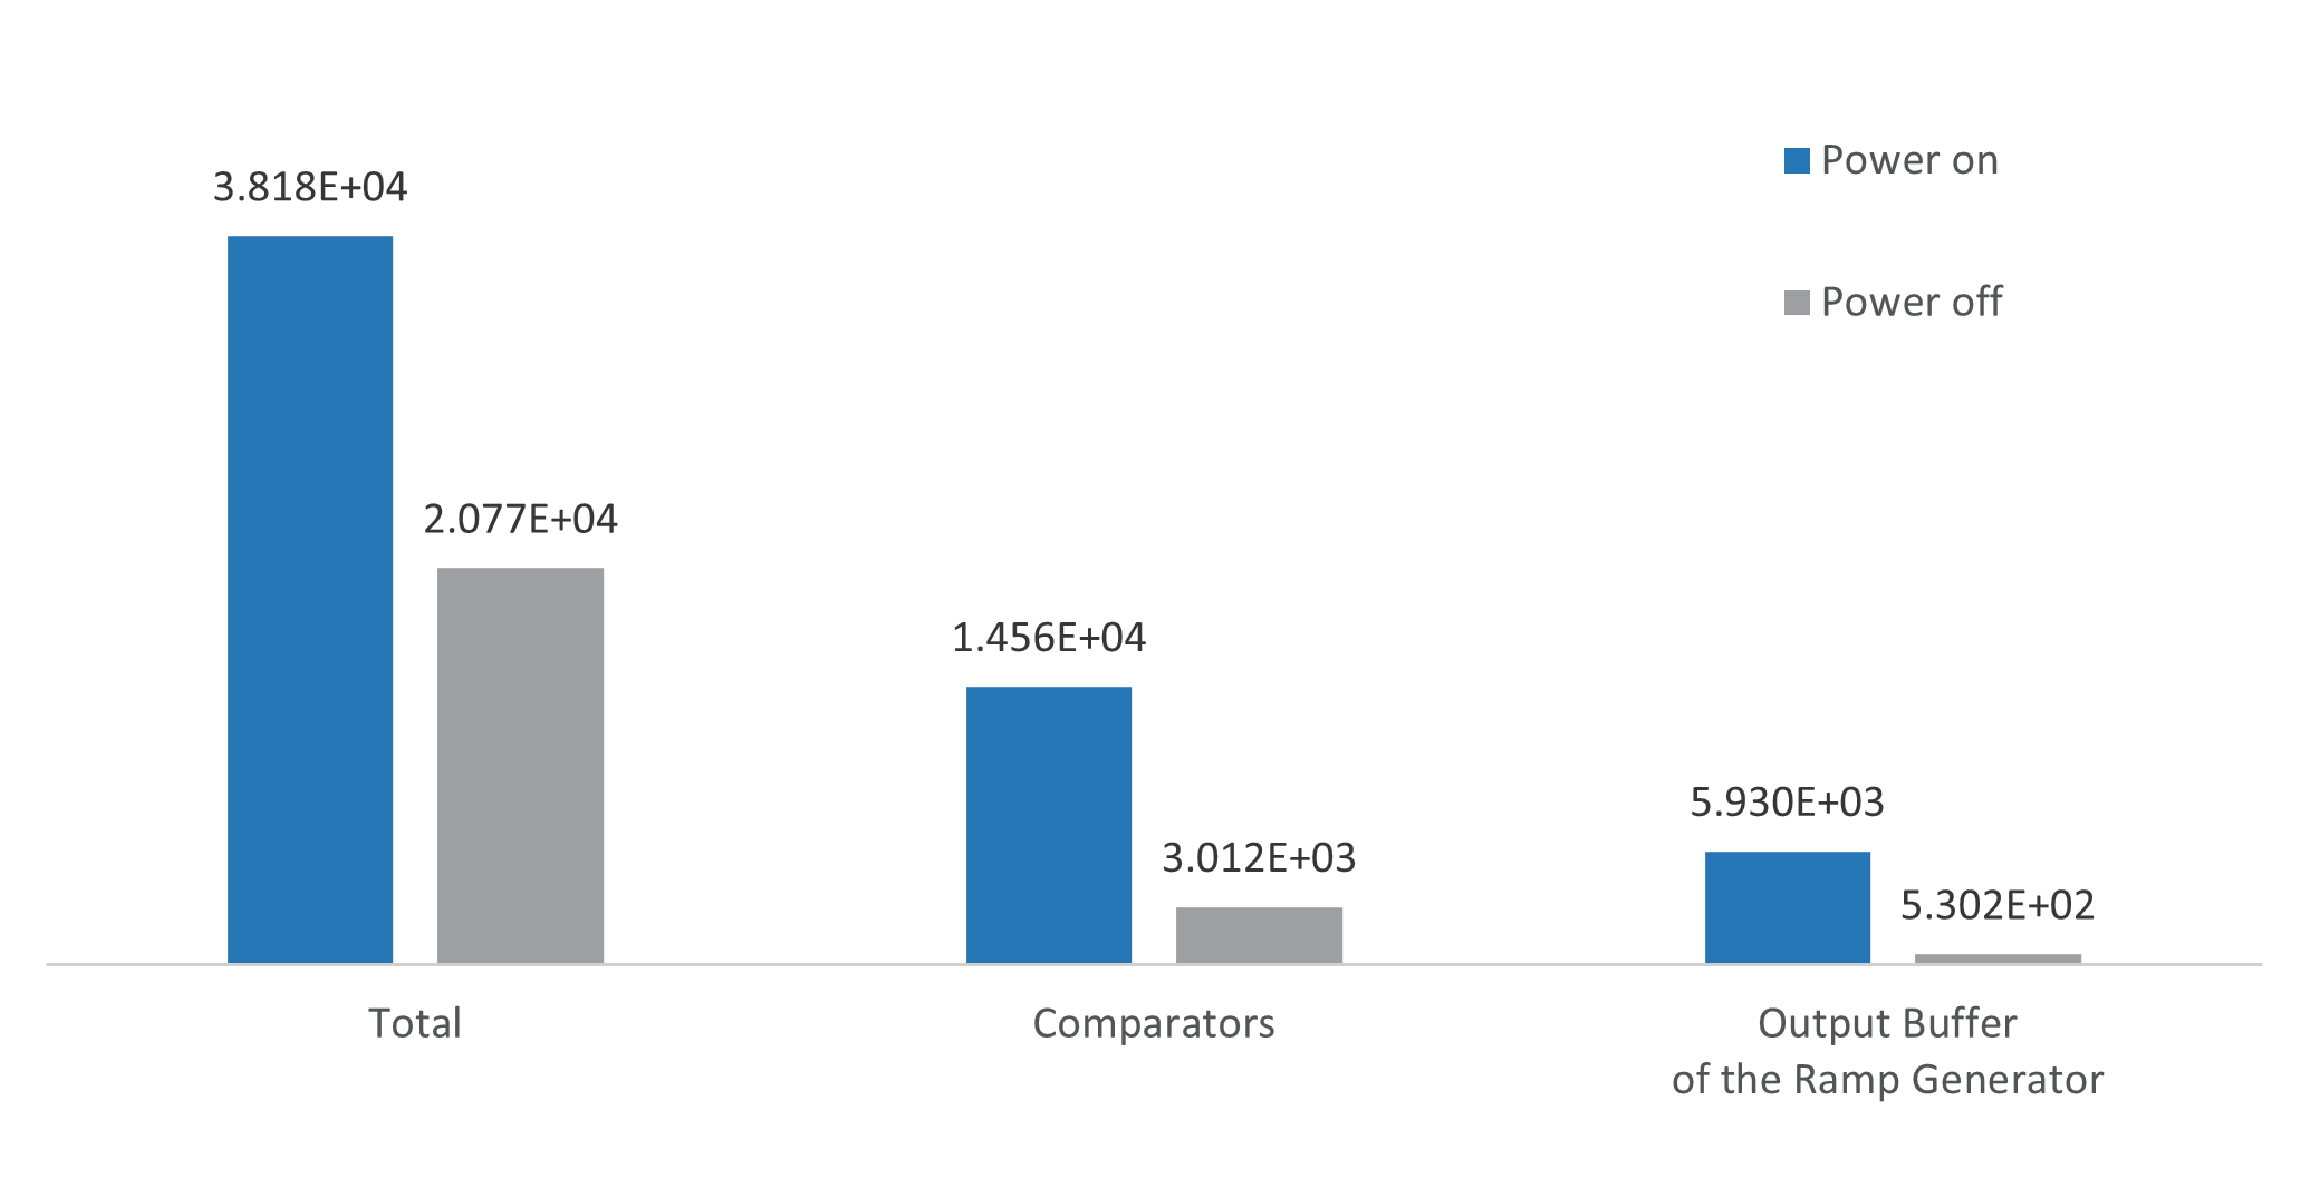
\includegraphics[width=3.5in]{./Figures/SSResults2.eps}}
	\caption{Power Saving Results of the SS ADC design.}
	\label{SSresults2}
\end{figure} 

\subsection{Evaluation of the SAR/SS ADC design}

Table~\ref{tab2} summarizes the key design characteristics of the SAR/SS ADC design, for which 
we consider the same setup as that of the SS ADC. Since fewer steps are required in the SAR/SS ADC 
design, 1 step is equivalent to 2 clock periods. The SNDR is 24.25/57.87 dB and the ENOB is 3.74/9.32 bits, 
which is inline with the design specifications. The power consumption of the SAR/SS ADC design is 256.1uW/column for the high-precision conversion mode and 137.1uW/column for the low-precision conversion mode. 
Compared to the high-precision conversion mode, the low-precision conversion mode can reduce the power 
consumption approximately 50\%. Detailed power breakdown is shown in Fig.~\ref{SARresults1}, which 
demonstrates that the power consumption of the SAR/SS ADC design is mainly contributed by the column-parallel buffers of the reference voltages in the sub-ADC, and power gating can effectively minimize the power consumption of these 
power-dominant components. The power consumption results are also presented in Fig.~\ref{SARresults2}.

\begin{table}[htbp]
	\caption{Performance of the SAR/SS ADC design}
	\begin{center}
		\begin{tabular}{|c|c|}
			\hline
			\textbf{Prameter}& \textbf{Value} \\
			\hhline{|==|}
			\textbf{Process}& 65nm \\
			\hline 
			\textbf{Supply voltage}& 2.5/1.2 V \\
			\hline
			\textbf{Clock Frequency}&	20MHz \\
			\hline
			\textbf{Architecture}&	SAR/SS \\
			\hline
			\textbf{Quantization bits}&	4/10 bits \\
			\hline
			\textbf{Conversion time (us)}&	10.1us \\
			\hline
			\textbf{Number of parallel columns}&	512 \\
			\hline
			\textbf{Throughput (samples per second)}&	50.7M \\ 
			\hline
			\textbf{Power (per column)}&	137.1/256.1 uW \\
			\hline
			\textbf{SNDR}& 24.25/57.87 dB@ 10.06 kHz \\
			\hline
			\textbf{ENOB}& 3.74/9.32 bits \\
			\hline
			\textbf{FOM$^{\mathrm{a}}$}& 103.64/4.05 pJ/step\\
			\hline
			\multicolumn{2}{l}{$^{\mathrm{a}}\textbf{FOM}=(\textbf{Power}\ast \textbf{Conversion}\ \textbf{time})/2^{\textbf{ENOB}}$ }	    
		\end{tabular}
		\label{tab2}
	\end{center}
\end{table}

\begin{figure}[htbp]
	\centerline{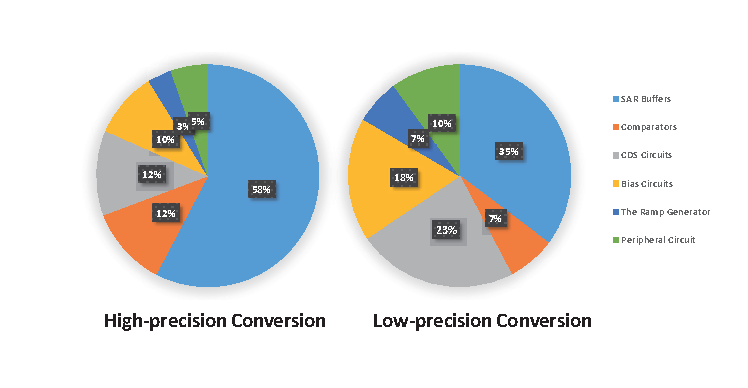
\includegraphics[width=3.5in]{./Figures/SARResults1.eps}}
	\caption{Power Distribution of the SAR/SS ADC design.}
	\label{SARresults1}
\end{figure} 

\begin{figure}[htbp]
	\centerline{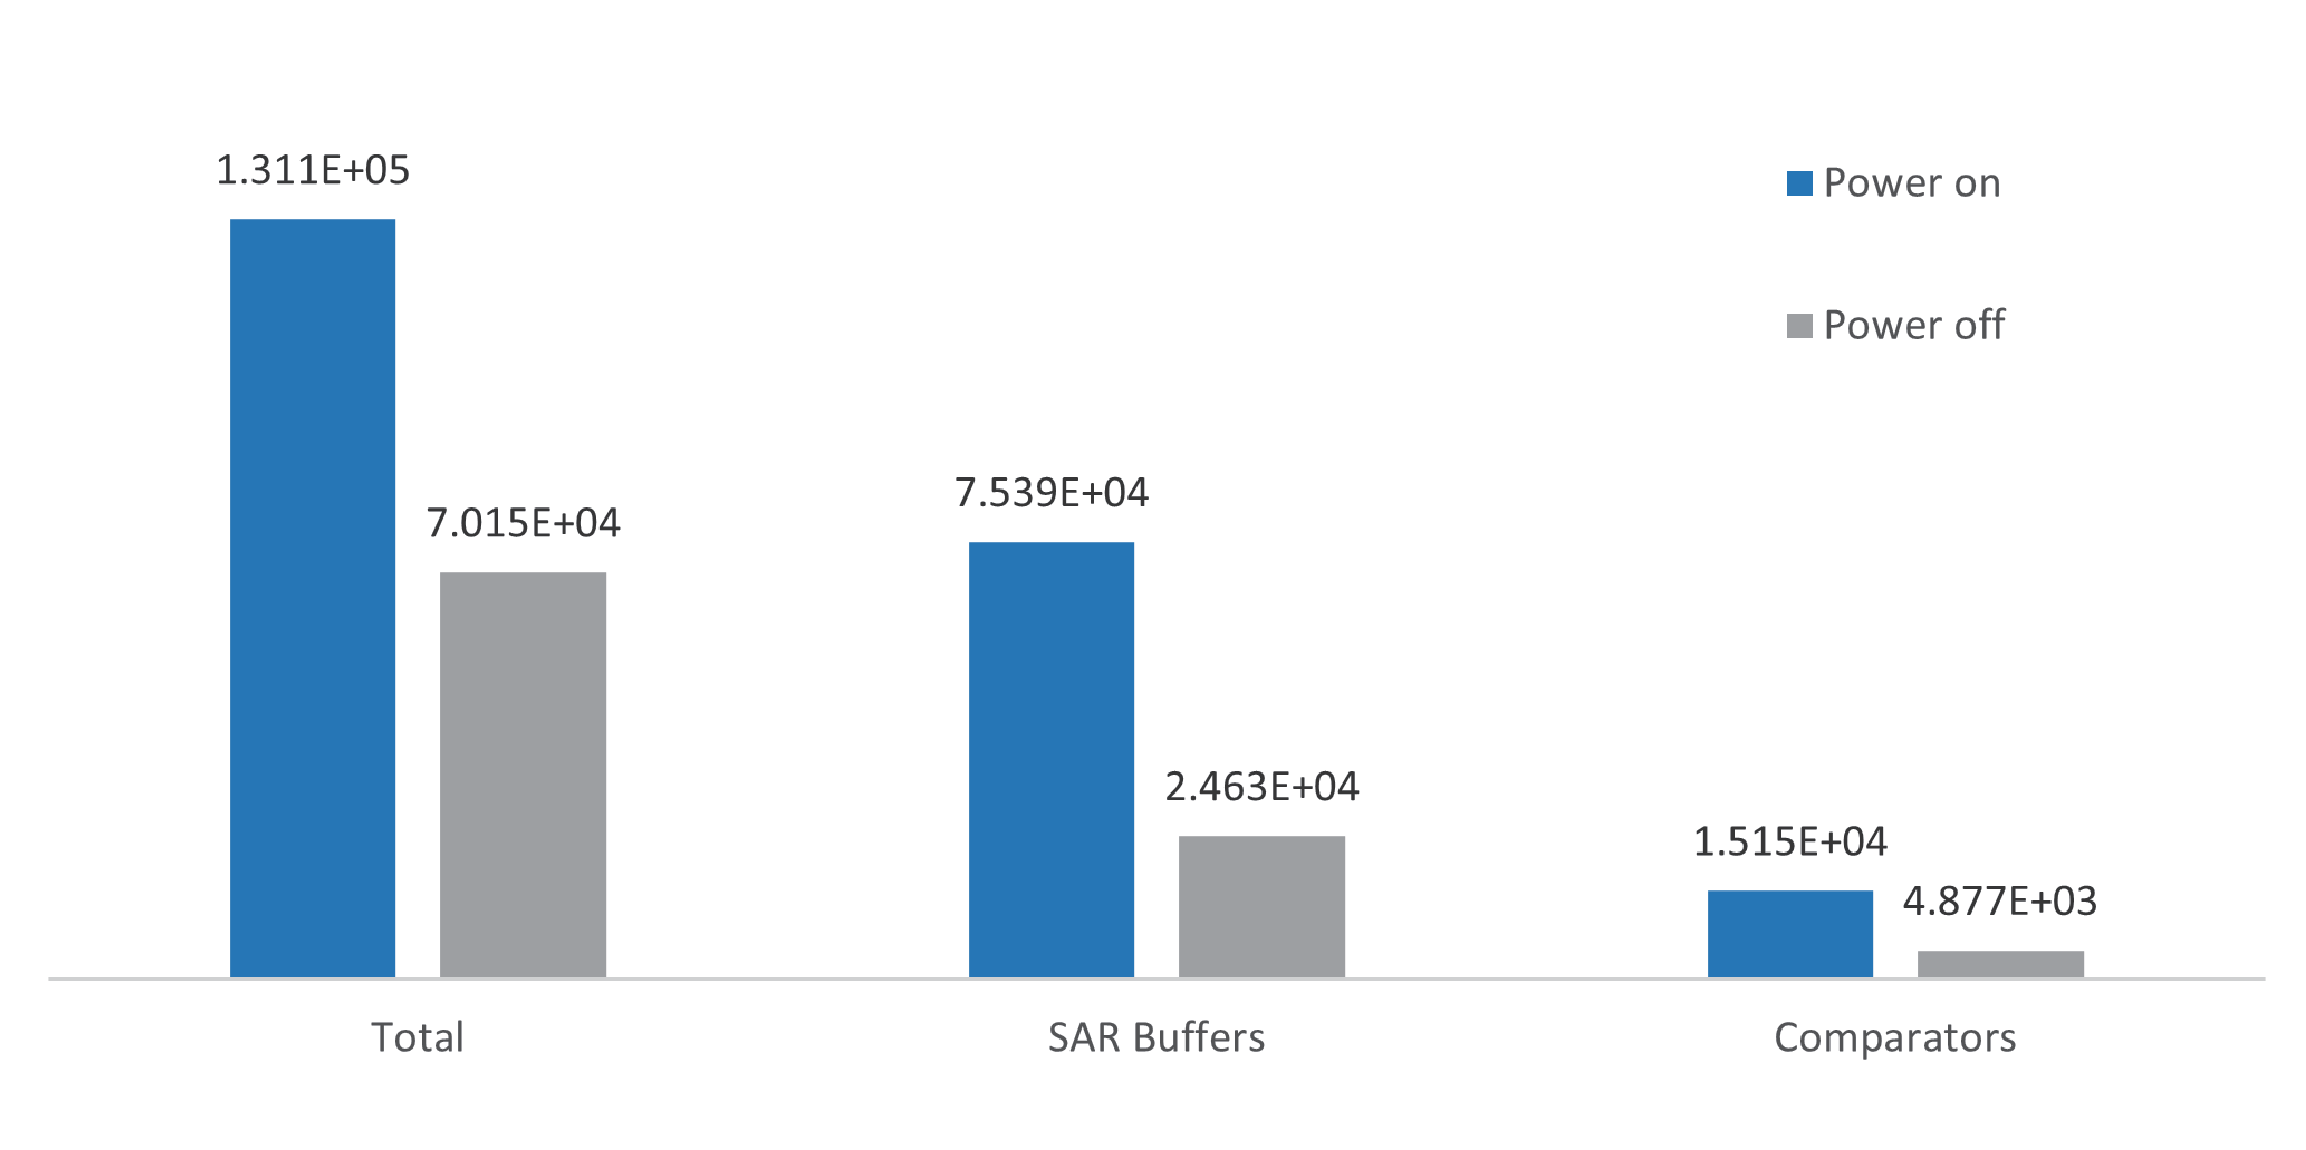
\includegraphics[width=3.5in]{./Figures/SARResults2.eps}}
	\caption{Power Saving Results of the SAR/SS ADC design.}
	\label{SARresults2}
\end{figure} 
